\documentclass[a4paper]{article}
\usepackage[left=2.1cm, right=2.1cm, top=2.1cm]{geometry}
\usepackage{lipsum}
\usepackage{tikzpagenodes}
\usepackage{pgfplots}
\usepackage{tikz}
\usepackage{tikz-3dplot}
\usetikzlibrary{arrows,decorations.pathmorphing,backgrounds,positioning,fit,matrix}
\pgfplotsset{compat=1.8}
\usepackage{graphics} % for pdf, bitmapped graphics files
\usepackage{epsfig} % for postscript graphics files
\usepackage[colorlinks=true,citecolor=green]{hyperref}
\usepackage{cite}
\usepackage{amsmath,amssymb,amsfonts}
\usepackage{algorithmic}
\usepackage{graphicx}
\usepackage{url}
\usepackage{cite}
\usepackage{bm}
\usepackage{pbox}
\usepackage{siunitx,booktabs,etoolbox}
\usepackage{ulem}
\usepackage[framed,numbered,autolinebreaks,useliterate]{mcode}
\usepackage{filecontents}
%\usepackage{bigfoot} % to allow verbatim in footnote


\def\BibTeX{{\rm B\kern-.05em{\sc i\kern-.025em b}\kern-.08em
    T\kern-.1667em\lower.7ex\hbox{E}\kern-.125emX}}


\begin{document}

\title{Exercise on RANSAC}
\author{xiahaa@space.dtu.dk}
\maketitle%%

In this exercise, you will work on RANSAC for line estimation and plane estimation.

\section{RANSAC}
\begin{itemize}
\item Read supplementary docs on RANSAC.
\item Implement $4$ main routines for RANSAC: 
\begin{enumerate}
\item random sampling a minimum set.
\item estimating model parameters.
\item compute consensus.
\item update iteration.
\end{enumerate}
\item Try your RANSAC with line and plane data.
\end{itemize}

\textbf{It is a good idea to organize your code as separate functions which can be reused.}

\begin{figure*}[!b]
\centering
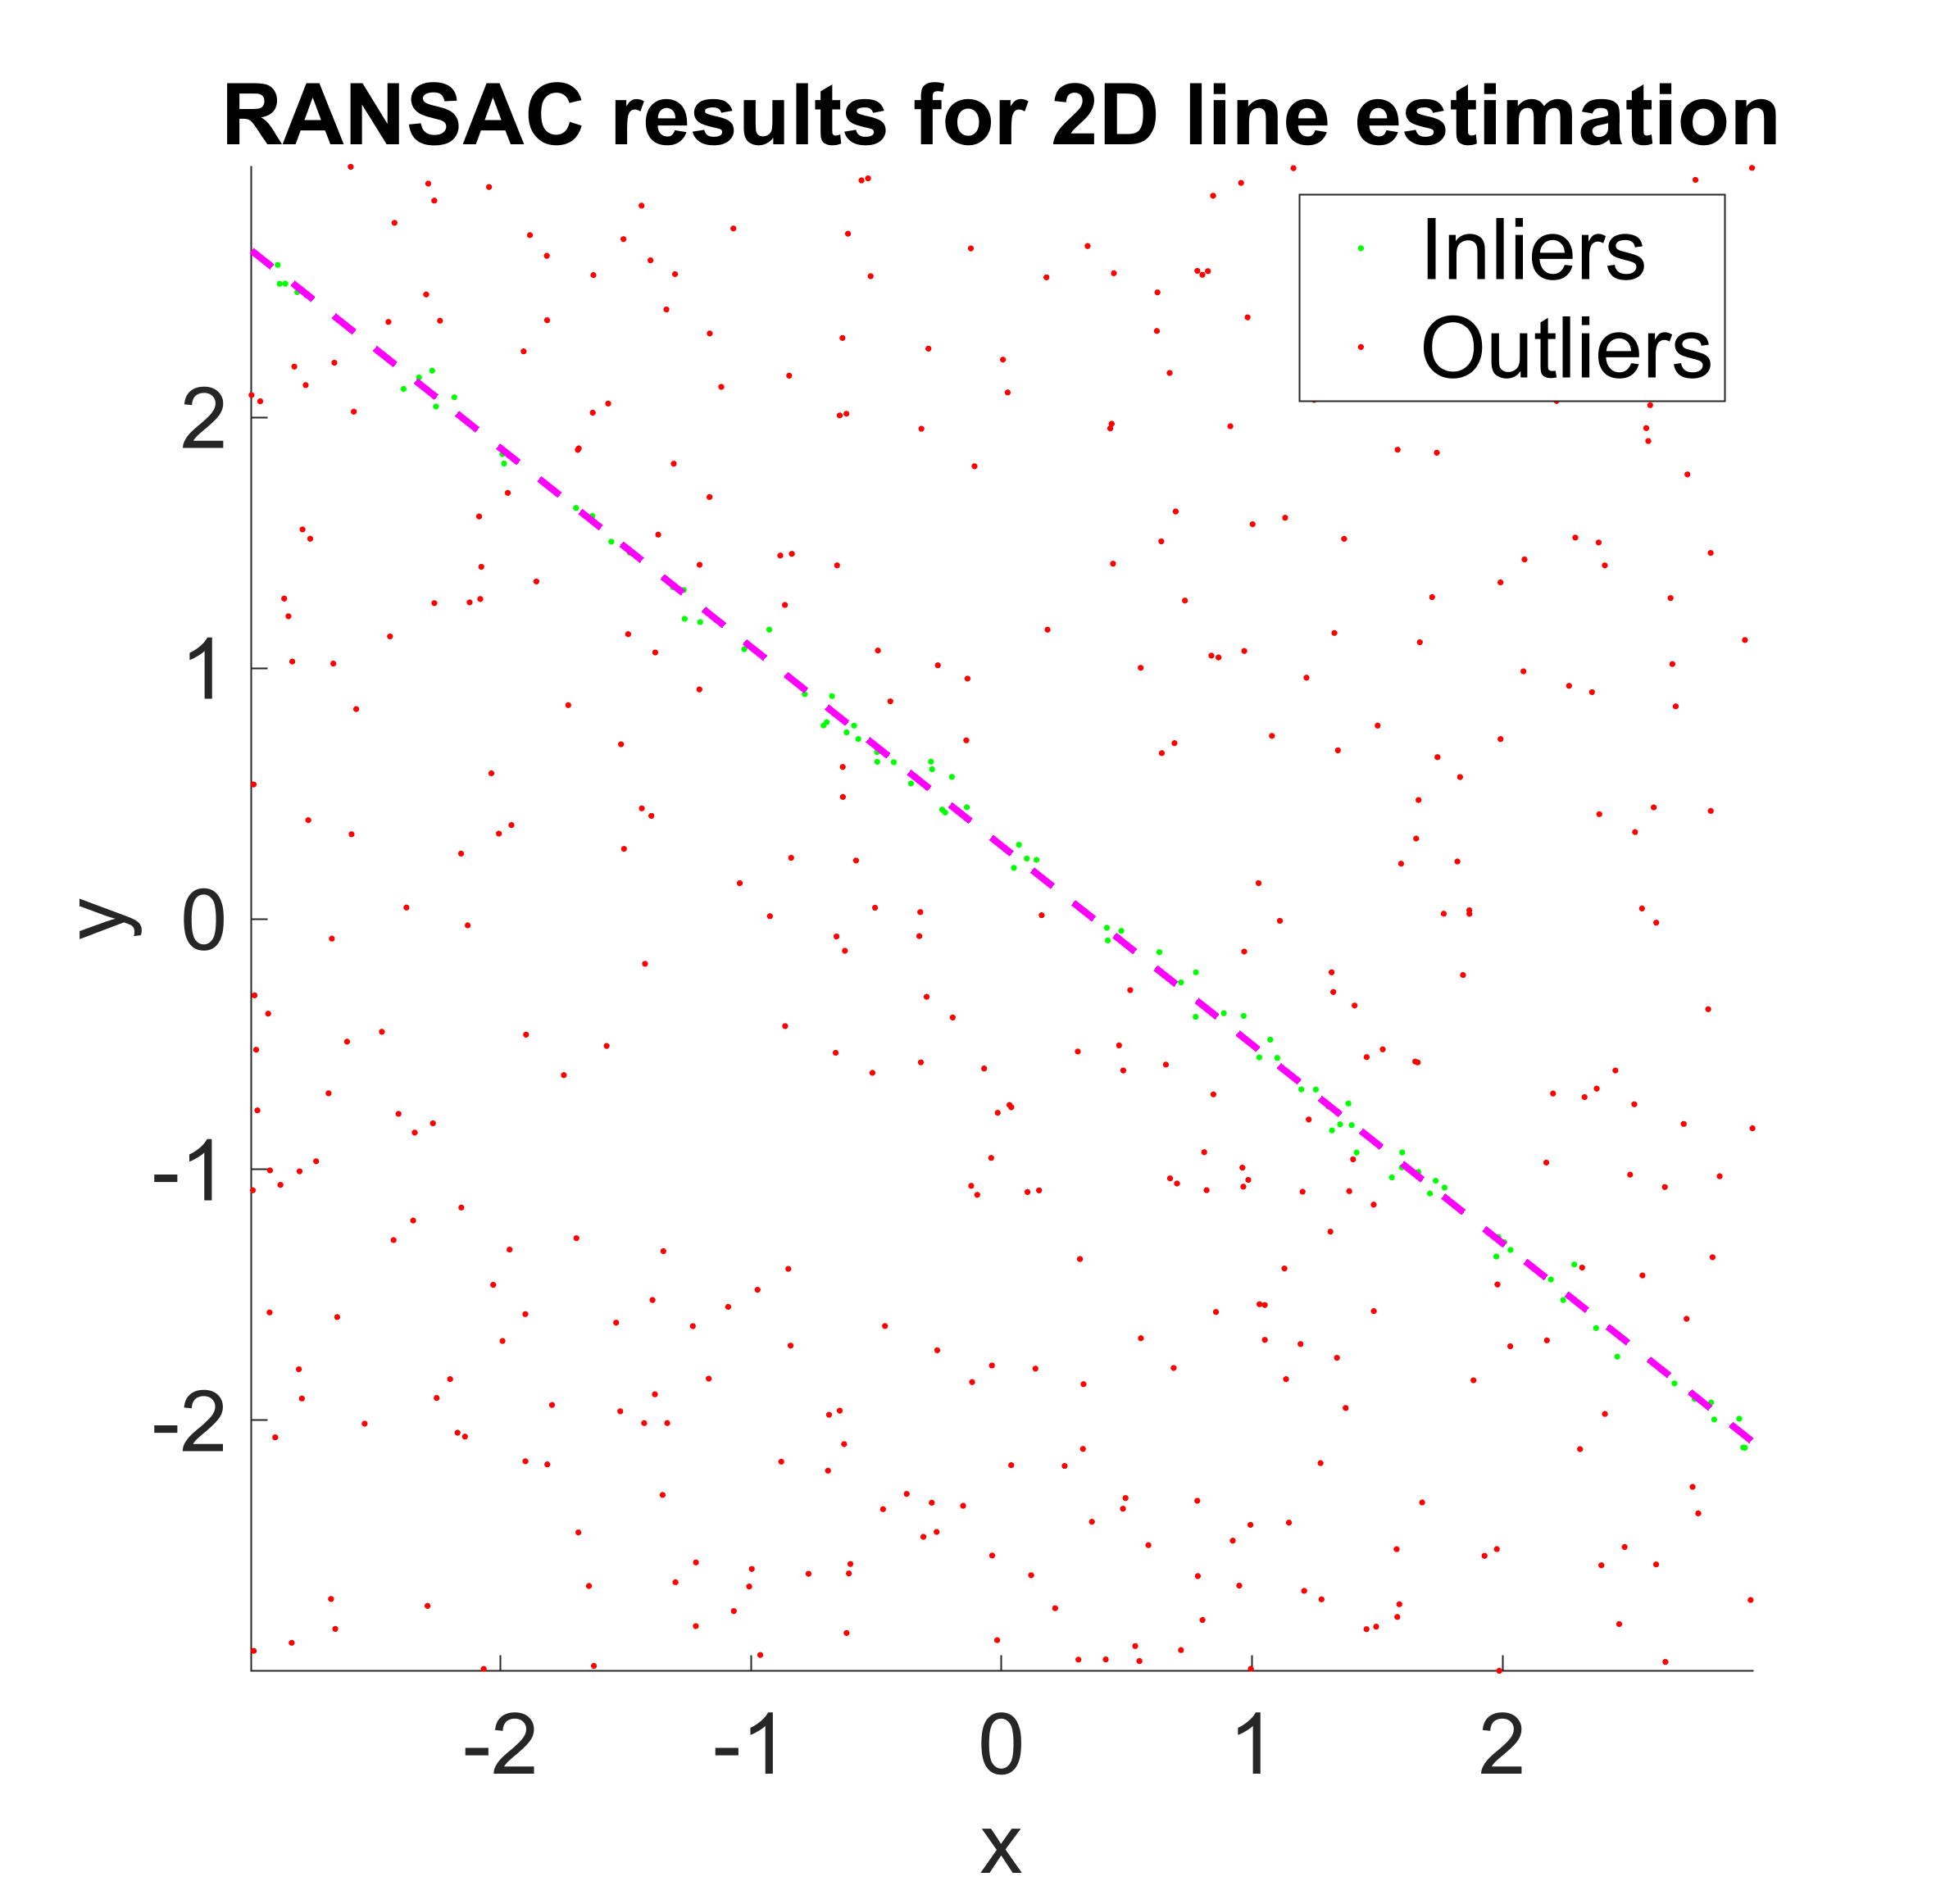
\includegraphics[scale=0.4]{figures/ransac_line.png}
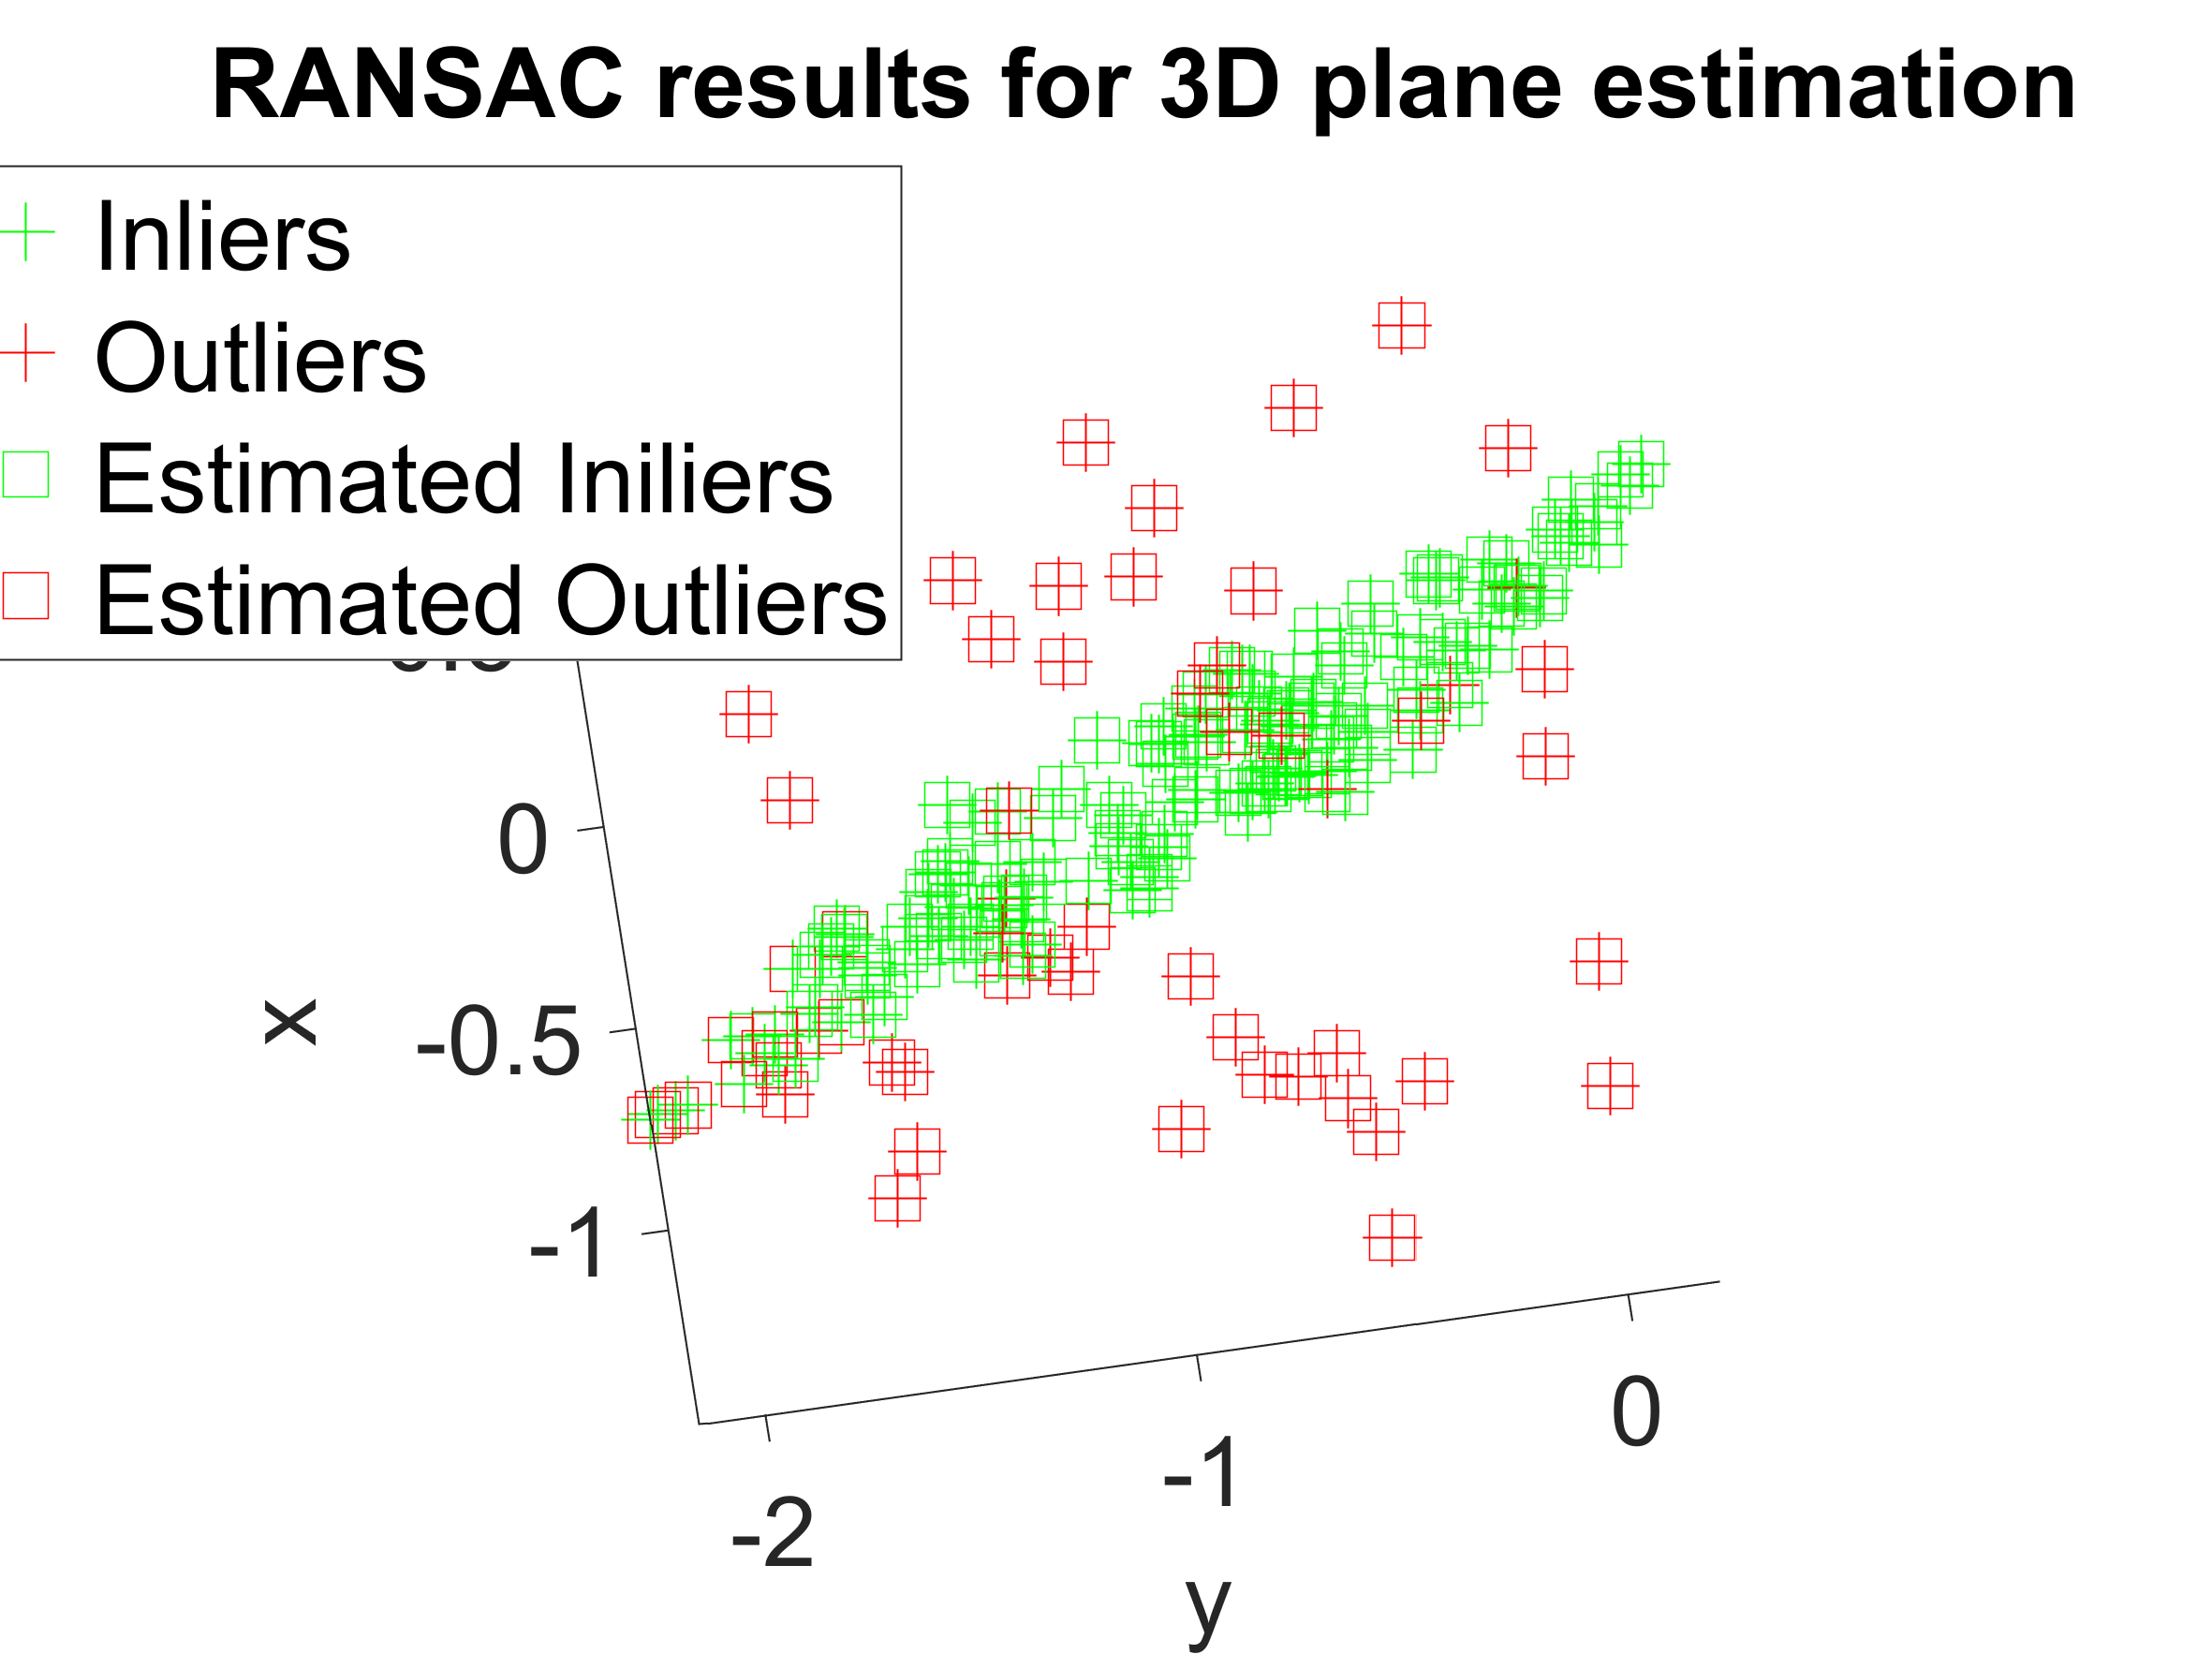
\includegraphics[scale=0.4]{figures/ransac_plane.png}
\caption{Example of RANSAC based line and plane estimation results.}
\end{figure*}

\end{document}